\chapter{Resultados obtidos}
\label{cap-resultados}
Este capítulo relata os resultados encontrados, a partir da proposta de
definição e preparação dos estudos, no Capítulo \ref{cap-metodologia}. Também dito 
no Capítulo \ref{cap-metodologia}, as aplicações escolhidas foram  
Owncloud; Wordpress; Moinmoin; Roundcube; e Noosfero. Além da aplicação de serviço
de e-mail.
 
Cada fase da implantação será tratada como uma 
subseção na descrição de cada aplicação que foi escolhida para exemplo de uso. 
Todas as atividades foram organizadas,
via \textit{issues}, no repositório do próprio projeto Shak 
\footnote{https://gitlab.com/shak/shak/issues}.

\section{Wordpress}
\label{sub:wordpress}

\citeonline{wordpress} é uma plataforma semântica de vanguarda para publicação pessoal, 
com foco na estética, nos padrões web e na usabilidade, ao mesmo tempo é 
um software livre. Além disso, Wordpress é um dos maiores softwares de 
publicação de conteúdo . 

Primeiramente, foram seguidos os procedimentos definidos na Seção 
\ref{section:construcao}. Para isso, era
necessário definir as fases e procedimentos da implantação automatizada,
seguindo as fases que compõem o processo proposto descrito na Seção \ref{sec:fases}.

\subsection{Planejamento}

Nesta fase foi preciso definir quais são as dependências mínimas
para o funcionamento da aplicação, tais como: banco de dados; pacotes
pré-instalados; e aplicações pré-configuradas. Para o Wordpress foram escolhidas:

\begin{itemize}
   \item \textbf{Pacote Wordpress para o Debian} 
   \item \textbf{Pacote Nginx para o Debian} 
   \item \textbf{Pacote MySQL para o Debian}
   \item \textbf{Arquivos de configuração:} Criação dos arquivos de configuração
   necessários para configurar o Wordpress, o servidor web Nginx e o banco de dados
   MySQL.
\end{itemize}

A instalação e execução desses recursos foram feitas nas fases seguintes.

\subsection{Preparação e Instalação de Pacotes}
\label{wordpress:preparacao}

Nesta fase foram definidos os procedimentos necessários para 
preparar o ambiente alvo, para que o Wordpress
possa ser executado. Isso envolveu a configuração do sistema operacional; instalação
e configuração de dependências necessárias; e a transferência do componente
para o servidor onde ele será executado.

Para esse procedimento, foi necessário instalar os pacotes \textit{php5-fpm}; o pacote
do banco de dados MySQL; e o pacote \textit{nginx}. Além disso, habilitar o serviço do
\textit{php5-fpm}.
 
Para executar essas instalações, foi preciso criar uma receita no livro de receitas
do Wordpress. Foi necessário criar o próprio livro de receitas no Shak.

Assim, com a estrutura gerada pelo rake, é possível declarar as dependências do Wordpress
dentro do arquivo \textit{default.rb}, dentro do diretório \textit{recipes}. Nesse 
arquivo, são declarados: os pacotes que devem ser instalados; os arquivos de configuração;
os serviços que precisam executar; os diretórios; e permissões de usuários. 

O código \ref{codigo998} é um exemplo de como declarar pacotes e serviços dentro de uma receita Chef.

\begin{lstlisting}[basicstyle=\ttfamily, language=Ruby,label=dice_index,caption={Exemplo de criação de serviço do mysql com o chef}, label=codigo998]
  package "mysql-server"
  service "mysql" do
    action :start
  end
\end{lstlisting}

\subsection{Configuração}
\label{wordpress:preparacao}

O primeiro arquivo de configuração é o \textit{config.php}. Esse arquivo contém a
configuração onde ficam as informações de banco de dados, como nome do banco de dados;
login do usuário do banco de dados; senha; o endereço do banco de dados. Além disso,
cada aplicação deve possuir um diretório
onde ficam os arquivos estáticos, como: temas; galeria de mídias; e plugins 
de cada instância do Wordpress.

Esse arquivo deve ficar no diretório \textit{/etc/wordpress/} e seu nome deve conter
a seguinte estrutura: \textit{config-nomehost.php}, onde o nomehost deve ser o endereço
desejado, como por exemplo config-fga.unb.br.php. O segundo arquivo é o \textit{database.sql}, que é um pequeno script \textit{SQL} que
cria o banco de dados do Wordpress e dá os privilégios ao usuário desejado. Por fim,
o arquivo de configuração do Nginx, com a configuração do servidor web.

Na receita chef, esses arquivos de configuração serão criados dentro do diretório 
\textit{template}, com o conteúdo dos arquivos de configuração. A ação que cria 
um arquivo na receita chef é 
declarada dentro do arquivo \textit{default.rb}, de forma semelhante como foi feito com
a declaração dos pacotes. 

O código \ref{codigo997} é um exemplo de como gerenciar templates numa receita Chef.

\begin{lstlisting}[basicstyle=\ttfamily, language=Ruby,label=dice_index,caption={Exemplo de criação de templates com o chef}, label=codigo997]

template "Create autoconfig.php in /etc/wordpress" do
  source "autoconfig.php.erb"
  path "/etc/wordpress/autoconfig.php"
  owner "www-data"
  group "www-data"
end
\end{lstlisting}

\subsection{Múltiplas Instâncias}

O Wordpress já suporta a funcionalidade de múltiplas instâncias nativamente. 
Para configurá-lo, foi necessário que alguns diretórios do Wordpress
fossem isolados, sendo um para cada aplicação. Cada instância precisa
ter seus diretórios isolados.

Outro fator importante é que, cada instância
tenha seu banco de dados. Para
solucionar esse problema, o Shak possui um recurso interessante, onde cada aplicação
possui um atributo \textit{id}, que é um atributo único para cada instância executada pelo
Shak. Com isso, foi possível criar diretórios personalizados com o id de cada aplicação, 
e também bancos de dados específicos e arquivos \textit{config.php} específicos.

Por fim, era necessário um arquivo de configuração Nginx para cada aplicação,
como visto no Capítulo \ref{cap-referencial}. Todo arquivo de configuração
do Nginx possui um bloco \textit{server}, e cada bloco \textit{server} equivale a uma hospedagem virtual. 
Por isso, as aplicações também se tornam independentes, podendo ser acessadas pelo 
mesmo servidor, mas com endereços diferentes. 

\subsection{Inicialização}

Após a construção da receita do Wordpress, foi necessário testar a receita construída. 
Para isso, o Shak precisa de duas informações importantes. A primeira, é a aplicação
que será instalada, e segunda, o endereço destino. Como a implantação foi um ambiente de desenvolvimento,
não é preciso configurar um ip ou configurar um \textit{DNS}. Foi preciso adicionar o
endereço desejado no arquivo \textit{/etc/hosts}. Assim, mesmo que esteja na sua máquina local, 
era possível acessar um endereço mais familiar em seu navegador. 

Um exemplo da execução da instalação via Shak é executando o comando
\textit{"shak install wordpress hostname=wordpress.dev"}. Assim, o 
Shak processa os dados informados, registrando os dados em seu repositório, e
inicia a instalação da aplicação, executando sua receita. Dessa forma, o 
Chef inicia: o processo de instalação dos pacotes; criação dos arquivos
de configuração; incia os serviços desejados.

Ao fim do procedimento, a aplicação estará pronta para uso no endereço escolhido,
é possível também verificar o estado atual da aplicação.

Para listar todas as aplicações que estão no repositório do Shak e verificar 
suas informações é preciso executar o comando \textit{"shak list"}. Assim, é 
possível verificar o endereço em que a aplicação está disponível, além do estado atual da aplicação.

Como dito na Seção \ref{subsection:validacao}, a validação da instalação foi feita
a partir da verificação do funcionamento das funcionalidades básicas da aplicação,
além de testar múltiplas instalações no mesmo servidor e verificar se todas as
aplicações instaladas eram acessíveis através do protocolo \textit{HTTPS}.

\section{Owncloud}
\label{sub:owncloud}

\citeonline{owncloud} é uma ferramenta para compartilhamento de arquivos, é um software 
livre em que é possível compartilhar
um ou mais arquivos e diretórios do seu computador na nuvem, e sincronizá-los com o seu
servidor Owncloud. Esses arquivos são imediatamente sincronizados com o servidor
e disponibilizados para outros dispositivos que utilizam o ambiente de trabalho
Owncloud ou aplicativo Android ou aplicativo IOS.

Owncloud é uma ferramenta que se assemelha a aplicações conhecidas, como Dropbox
\footnote{https://www.dropbox.com/pt\_BR/} e Google Drive \footnote{https://www.google.com/intl/pt-BR/drive/}, porém, por ser software livre, é possível instalar Owncloud em servidores
que o usuário preferir. Em alguns casos, usuários criam nuvens privadas com 
owncloud, em pequenos servidores configurados em casa.

Para a ferramenta Owncloud, foram seguidos os mesmos passos feitos na aplicação
Wordpress na Seção \ref{sub:wordpress}.

\subsection{Planejamento}

As dependências para o funcionamento do Owncloud são:

\begin{itemize}
   \item \textbf{Pacote Owncloud para o Debian}
   \item \textbf{Pacote Nginx para o Debian}
   \item \textbf{Pacote Postgresql para o Debian}
   \item \textbf{Arquivos de configuração:} Criação dos arquivos de configuração
   necessários para configurar o Owncloud, o servidor web Nginx e o banco de dados
   Postgresql.
\end{itemize}

Diferentemente da aplicação Wordpress, na aplicação Owncloud o 
banco de dados escolhido foi o postgresql. Na documentação do Wordpress é recomendado
o uso do banco de dados MySQL, porém no Owncloud fica à escolha do desenvolvedor.
A escolha do Postgresql teve como motivação, a possibilidade de trabalhar com dois bancos de
dados diferentes, aumentando o suporte do Shak. Assim, quando existirem aplicações
que suportam apenas o Postgresql, o Shak já terá uma estrutura pronta.

\subsection{Preparação e Instalação de Pacotes}

Para esse procedimento, foi necessário instalar os pacotes \textit{php5-fpm}; o banco
de dados Postgresql; e o pacote Nginx. Além disso, habilitar o serviço do php5-fpm. 
Também foi necessário instalar o pacote php5-pgsql, que é um módulo para
conexões de banco de dados Postgresql, necessário para o funcionamento de
aplicações na linguagem PHP com o banco de dados Postgresql.

Para executar essas instalações, foi preciso criar uma receita no livro de receitas
do Owncloud, da mesma forma que em Wordpress.

Com a estrutura inicial, foi possível declarar as dependências do Owncloud
dentro do arquivo \textit{default.rb}, que se encontra dentro do diretório 
\textit{recipes}.
 
\subsection{Configuração}

O primeiro arquivo de configuração é o \textit{autoconfig.php}, esse arquivo
contém informações importantes, como: nome do banco de dados;
login do usuário do banco de dados; senha do usuário do banco de dados; o endereço 
do banco de dados; o diretório
onde irá ficar os arquivos de configuração do Owncloud; e o login e senha
do administrador. 

Além disso, foi necessário criar o diretório de conteúdos públicos do Owncloud, que por
padrão devem ficar em \textit{/etc/owncloud}. O segundo arquivo é o 
\textit{postgresql-conf.sql}, que é um pequeno script \textit{SQL} que cria o 
banco de dados do Owncloud, e configura os
privilégios ao usuário desejado. Por fim, a configuração do servidor web, feitos
através de templates, da mesma forma que a aplicação Wordpress.

\subsection{Múltiplas Instâncias}

Diferentemente do Wordpress, o Owncloud não suporta nativamente múltiplas instâncias. 
Porém isso não foi um impeditivo na execução do trabalho, com uma busca, encontrou-se uma 
discussão no repositório oficial do Owncloud relacionado a implementação dessa 
funcionalidade. 

Foi discutido uma proposta \footnote{https://github.com/owncloud/core/pull/16424} 
de solução que permitiria a configuração de múltiplas instâncias. O
resultado desta discussão foi que, os desenvolvedores do Owncloud não acharam relevante
a funcionalidade, mas caso o desenvolvedor ache necessário, ele poderia fazer essa
alteração diretamente no código fonte.

Porém, manter isso no Shak não seria uma boa solução. Uma solução para esse problema seria, 
enviar uma contribuição ao pacote do Owncloud no Debian, onde assim a contribuição feita
poderia ser facilmente utilizada por mais pessoas que queiram essa funcionalidade,
bastando utilizar a versão disponibilizada nos servidores do Debian. 

Com isso, foi feita a contribuição que adicionaria a funcionalidade de múltiplas 
instâncias para o Owncloud, e enviado ao mantenedor do pacote do Owncloud no Debian. 
Na discussão \footnote{https://bugs.debian.org/cgi-bin/bugreport.cgi?bug=789726},
a contribuição foi bem vista pelo mantenedor do pacote.
 
Os procedimentos feitos para suportar múltiplas instâncias
no Owncloud são bem semelhantes aos do Wordpress, criando um diretório de dados
para cada aplicação; um arquivo de configuração para cada aplicação; e um banco de
dados para cada aplicação. Seguindo a mesma abordagem do Wordpress, também
foi criada uma hospedagem virtual para cada instância do Owncloud.

\subsection{Inicialização}

A inicialização da aplicação se dá da mesma forma que na aplicação Wordpress.

Para executar a instalação do Owncloud basta executar o comando \textit{"shak install owncloud hostname=owncloud.dev"}.

A validação da instalação foi feita conforme dito na Seção \ref{subsection:validacao}, 
da mesma forma que em Wordpress.

\section{Servidor de e-mail}
\label{sub:e-mail}

Tanto Owncloud como Wordpress, possuem funcionalidades que utilizam serviços 
de e-mail. Assim, a construção de um servidor de e-mail 
possui bastante relevância, para que qualquer aplicação que precisar de um 
servidor de e-mail, possa utilizar o servidor de e-mail que o Shak possa fornecer.

Para adicionar o suporte a servidor de e-mail, também foram seguidos os mesmos passos
feitos no Wordpress na Seção \ref{sub:wordpress} e no Owncloud na Seção\ref{sub:owncloud}. 

\subsection{Planejamento}

Primeiramente, foi definido que o protocolo escolhido fosse o protocolo \textit{IMAP}, já
que o protocolo \textit{IMAP} é um protocolo online, ou seja, ele se conecta ao servidor
e realiza o download das mensagens, depois ainda  mantém a conexão para que
as alterações e mensagens novas sejam atualizadas em tempo real. Diferentemente do
protocolo \textit{POP3} que é um protocolo offline, onde após o download das mensagens encerra
a conexão. Outra vantagem do \textit{IMAP} em relação ao \textit{POP3}, é que o 
\textit{IMAP} mantém uma cópia de mensagens no servidor, ideal para quem precisa 
acessar os e-mails de mais de um local ou a partir de mais de um dispositivo.

O servidor \textit{IMAP} escolhido foi o Dovecot, que é um servidor de e-mail
\textit{IMAP}, além disso, Dovecot é um software livre simples de configurar, não requer 
administração especial, e ainda usa muito pouca memória \cite{dovecot}. 

O agente de transferência de e-mails escolhido foi o Postfix, que é um software
livre para envio e entrega de e-mails. A sua escolha foi feita pela facilidade de
integração com o Dovecot. Postfix é o software responsável pelo método de entrega de e-mail
utilizando \textit{SMTP}, como protocolo de transferência de e-mails. 

Por fim, a aplicação que servirá como anti-spam será o Apache SpamAssassin, que 
é uma plataforma anti-spam que dá aos administradores de servidor de e-mail, 
um filtro para classificar e-mails e bloquear os e-mails que julgarem como spam \cite{spam}. 

Em resumo, o servidor de e-mail é composto de:

\begin{itemize}
   \item \textbf{Pacote Dovecot para o Debian}
   \item \textbf{Pacote Postfix para o Debian}
   \item \textbf{Pacote spamassasin para o Debian}
   \item \textbf{Arquivos de configuração} Criação dos arquivos de configuração
   necessários para configurar o Spamassasin, Dovecot e Postfix.
\end{itemize}

\subsection{Preparação e Instalação de Pacotes }

Nesta fase foi necessário separar as dependências dos pacotes para cada ferramenta
escolhida, para compor o servidor de e-mail. Primeiramente, para o Postfix, são necessários
os pacotes \textit{postfix} e \textit{bsd-mailx}, além de habilitar o serviço do 
Postfix. Para o Dovecot,
foi necessário instalar o pacote \textit{dovecot-imadp} além de habilitar o serviço do Dovecot. 
Para o Spamassassin, eram necessários os pacotes \textit{spamassassin} e o pacote
 \textit{spamc}, além de habilitar o serviço do Spamassassin.

Na receita do servidor de e-mail, cada aplicação possui a sua receita específica,
e o arquivo \textit{default.rb}, que contêm a receita do servidor de e-mail. 

Esse arquivo contém apenas a chamada das receitas das aplicações, como no código \ref{codigo999}:

\begin{lstlisting}[basicstyle=\ttfamily, language=Ruby,label=dice_index,caption={Exemplo da receita de e-mail
composta pelas receitas das outras aplicações}, label=codigo999]
include_recipe 'email::dovecot'
include_recipe 'email::postfix'
include_recipe 'email::spamassasin'
\end{lstlisting}

A função de \textit{include\_recipe} do Chef permite que, aplicações que são compostas
por outras aplicações menores, possam ter suas receitas separadas em diferentes arquivos,
sendo uma receita para cada aplicação menor, que compõe o todo. Com isso, foi possível 
incluir esses arquivos na receita que será executada. No caso do Shak, a receita
que sempre será executada é a receita que está no arquivo \textit{default.rb} no diretório \textit{recipe}.

\subsection{Configuração}

Primeiramente, para a configuração do Dovecot, foram utilizados 5 arquivos
de configuração, o primeiro é o \textit{10-mail.conf} que é um arquivo de configuração para
indicar onde é o local no qual os e-mails estão. O segundo arquivo, é o \textit{10-ssl.conf}
que é o arquivo em que possui os caminhos do certificado \textit{SSL} e da chave \textit{SSL}.

O terceiro arquivo é o arquivo \textit{11-postfix-auth.conf}, arquivo responsável por 
indicar o caminho do arquivo de autenticação
do Postfix. O quarto arquivo é o arquivo \textit{20-imap.conf}, onde é indicado o tamanho
máximo de conexões por ip permitidas no servidor. Por fim, o arquivo
\textit{20-disable-imap-non-ssl.conf}, que permitirá que o imap utilize sempre uma conexão
segura utilizando o protocolo \textit{IMAPS} (\textit{IMAP} + \textit{SSL}), assim bloqueando 
qualquer conexão segura ou tentativa de conexão insegura.

Para o posfix, são apenas dois arquivos de configuração, o \textit{main.cf} e o 
\textit{master.cf}.
O \textit{main.cf} é onde se configuram os parâmetros mínimos de configuração, esse arquivo
também contém as configurações que filtram os e-mails com Spamassassin e 
algumas configurações do \textit{SMTP}. 

No \textit{master.cf}, é definido como um programa cliente se conecta a um serviço, e qual
programa é executado quando um serviço é solicitado. Neste caso, foi necessário
indicar que o servidor de e-mail utilize \textit{SSL}, com autenticação segura, 
apontando o caminho dos arquivos de chave e certificados.

Por fim, a configuração do Spamassasin. São necessários dois arquivos de configuração.
O arquivo \textit{spamassassin}, que é o arquivo de configurações padrão para o Spamassasin e o
\textit{local.cf} que são as configurações locais. No Spamassassin, foi preciso habilitar 
o serviço do Spamassasin e configurar o caminho dos arquivo de log.

Já o arquivo \textit{local.cf}, possui o parâmetro required\_score. Esse parâmetro 
possui um nível de 0 a 10, em que 
são classificados os e-mails como spam. Por padrão, esse valor é cinco. Porém, se 
o usuário quiser aumentar o filtro, é necessário aumentar para valores como seis ou sete, 
até chegar em um nível de confiança em que o spamassasin cuide dos casos falsos-positivos, 
ou seja, e-mails que não são spam, porém foram interpretados como spam.

\subsection{Inicialização}

A inicialização da aplicação se dá da mesma forma que nas aplicações Wordpress
e Owncloud.

Para executar a instalação do servidor de e-mail basta executar o comando \textit{
shak install e-mail hostname=owncloud.dev}

Para testar o funcionamento, foram feitos dois procedimentos. O primeiro, era utilizar
um cliente de e-mail para testes. O cliente de e-mail escolhido foi o mutt, utilizando
suas funções básicas de enviar e receber e-mails. O segundo passo, foi realizar conexões
com o servidor de e-mail via comando \textit{telnet}. 

Para isso, foi necessário executar os seguintes comandos: \textit{telnet localhost imap} e
\textit{telnet localhost imaps}. Pela configuração do servidor de e-mail, não foi possível abrir uma conexão 
\textit{telnet}
com o parâmetro \textit{imap}, porém com o parâmetro \textit{imaps} foi possível, isso serviu para testar 
que o servidor de e-mail impediu conexões que não 
utilizam os protocolos criptografados.

\section{Moinmoin}
\label{sub:moinmoin}

\cite{moin} é uma ferramenta de construção
de wikis, com uma grande comunidade de usuários, podendo criar páginas web
facilmente editáveis. Moinmoin é software livre. Alguns exemplos
de wiki que utilizam o Moinmoin são: Wiki do Debian, Wiki do Python e Wiki do Apache,
contendo várias documentações relacionadas aos seus softwares. 

Para a implantação automatizada do Moinmoin, foram seguidos os mesmos passos
feitos em Wordpress \ref{sub:wordpress} e Owncloud \ref{sub:owncloud}.

\subsection{Planejamento}

As dependências necessárias para a aplicação Moinmoin são:

\begin{itemize}
   \item \textbf{Pacote python-moinmoin para o Debian}
   \item \textbf{Pacote Nginx para o Debian}
   \item \textbf{Pacote uwsgi para o Debian}
   \item \textbf{Arquivos de configuração:} Criação dos arquivos de configuração
   necessários para configurar o Uwsgi, o servidor web Nginx e o servidor web
uwsgi.
\end{itemize}

Diferentemente das outras aplicações web, Moinmoin não utiliza banco de dados.

\subsection{Preparação e Instalação de Pacotes}

Para esse procedimento, foi necessário instalar os pacotes \textit{uwsgi},
\textit{uwsgi-plugin-python}, e o pacote do Moinmoin, chamado \textit{python-moinmoin}.
Para executar essas instalações, foi preciso criar uma receita no livro de receitas
do Moinmoin.

Assim, com a estrutura inicial, foi possível declarar as dependências do Moinmoin
dentro do arquivo \textit{default.rb} dentro do diretório \textit{recipes}.

\subsection{Configuração}

O primeiro arquivo de configuração é o \textit{moin.wsgi}, arquivo onde é necessário
informar, por exemplo, o caminho dos arquivos de configuração do Moinmoin. No caso
de um pacote Debian, esse caminho por padrão é  \textit{/etc/moin}. Também foi necessário 
editar o arquivo \textit{uwsgi.ini}, que é o arquivo de configuração
do uwsgi para a sua aplicação. Nele, foi possível adicionar informações importantes, como
por exemplo: caminho do arquivo de log do uwsgi; caminho do socket;
e a quantidade máxima de requisições.

O terceiro arquivo de configuração é o \textit{mywiki.py}, onde foi necessário
informar informações básicas da wiki, como o nome da wiki e seu diretório de dados. 
O último arquivo de configuração é o \textit{farmconfig.py}, que é o responsável pelos 
links da barra de navegação e responsável por configurar múltiplas instâncias.

Além disso, foi necessário criar o diretório de conteúdos do Moinmoin, que por
escolha devem ficar em /var/lib/moin. Após isso, para que o Nginx funcione corretamente
com o uwsgi, foi necessário indicar o socket do uwsgi, que foi indicado no uwsgi.ini.

\subsection{Múltiplas Instâncias}

Moinmoin possui nativamente a funcionalidade que permite a criação de múltiplas 
instâncias de wiki no mesmo servidor. Para isso, foi necessário editar um arquivo,
que é chamado de \textit{farmconfig.py}, com todas as wikis, e com seus 
respectivos identificadores e domínios. Assim, o Moinmoin consegue gerenciar as 
wikis separadamente. 

Uma outra etapa, era fazer com que o Shak entenda que existem outras wikis já 
configuradas. A cada nova instância
o arquivo \textit{farmconfig.py} deve ser atualizado com as novas 
informações de wiki, sem remover as
informações das outras wikis anteriormente inseridas. Para isso, foi adicionado
numa lista de wikis, para que a cada vez que surja uma wiki nova, apenas as
informações novas são inseridas no arquivo \textit{farmconfig.py}.

\subsection{Inicialização}

A inicialização da aplicação se dá da mesma forma que nas aplicações Wordpress
e Owncloud.

Para executar a instalação do Moinmoin executar o comando \textit{shak install moinmoin hostname=moinmoin.dev}. 
A validação da instalação foi feita conforme dito na Seção \ref{subsection:validacao}, 
da mesma forma que em Wordpress e Owncloud.

\section{Outras Aplicações}
\label{sub:appnencerradas}

Até o fim deste trabalho, as aplicações Noosfero e Roundcube não foram finalizadas. 
Porém, é importante reportar o estado atual do que foi feito até o momento,
com essas duas aplicações.

\subsection{Noosfero}
\label{subsub:noosfero}

\citeonline{noosfero} é uma plataforma web para redes sociais e 
de economia social e solidária. Ela possui funcionalidades como blog; e-Portfolios; 
CMS; RSS; discussão temática; agenda de eventos; e inteligência coletiva para a 
economia solidária no mesmo sistema.

O estado atual da aplicação Noosfero no Shak encontra-se
na fase do planejamento. No planejamento, já era de conhecimento do autor que o
Noosfero não estava nos repositórios oficiais do Debian, mas que seria possível estar, 
desde que todas as dependências do Noosfero também estivessem no Debian.

O Noosfero já possui um repositório \footnote{http://download.noosfero.org/debian/jessie/}
com suas dependências empacotadas. Porém, algumas delas não se encontram nos repositórios
oficiais do Debian, dificultando assim, que o pacote do Noosfero fique disponível
nos repositórios oficiais do Debian. 

Um exemplo é a biblioteca \textit{ruby-selenium-webdriver}, que
está no repositório do Noosfero, porém, ela não está disponível no repositório oficial
do Debian. Outro problema que foi encontrado, é que algumas dependências do Noosfero
estão em versões diferentes das dependências que estão no repositório Debian.

Para resolver esse problema, seria necessário empacotar todas as dependências
do Noosfero que ainda não estão no Debian. Além disso, sincronizar as versões
que já estão no Debian, com as versões que são utilizadas pelo Noosfero.

Na tabela \ref{tabela1} em anexo, encontra-se uma lista das dependências 
que estão no repositório do Noosfero,
com suas versões, e as dependências que estão no Debian Jessie.

Como visto na tabela \ref{tabela1}, grande parte das dependências do Noosfero encontram-se
 apenas nas versões \textit{testing} e \textit{unstable} no Debian. Para continuar com
a implantação automatizada, seria necessário discutir alguma solução 
com a comunidade do software. 

Como sugestão, uma das soluções viáveis seria 
sincronizar as versões das dependências do Noosfero, com as versões que são 
disponibilizadas pelo Debian \textit{testing}. Com isso, o 
Noosfero passa a ter boa parte de suas dependências suportadas pelo Debian. Além disso, 
também seria necessário empacotar as bibliotecas do Noosfero que o Debian não possui. 

Porém, essa decisão fica a cargo da comunidade da aplicação, e com o Noosfero disponível
nos repositórios oficiais do Debian, o Shak poderá dar suporte ao Noosfero, 
em trabalhos futuros.

 \subsection{Roundcube}
\label{sub:owncloud}

\citeonline{roundcube} é uma solução de webmail gratuita, de código 
aberto. Possui uma interface funcional e personalizável. Com ele, é possível
ler seus e-mails a partir de um cliente web. 

Para a ferramenta Roundcube, foram seguidos os mesmos passos feitos em 
\ref{sub:wordpress} e \ref{sub:owncloud}.

As dependências identificadas foram:

\begin{itemize}
   \item \textbf{Pacote Roundcube para o Debian}
   \item \textbf{Pacote Nginx para o Debian}
   \item \textbf{Pacote Postgresql para o Debian}
   \item \textbf{Arquivos de configuração:} Criação dos arquivos de configuração
   necessários para configurar o Roundcube, o servidor web Nginx e o banco de dados
   Postgresql.
\end{itemize}

Para facilitar a configuração de aplicações PHP, foi feito uma receita genérica
que instala dependências básicas para qualquer aplicação PHP que for usada pelo
Shak. Essa receita instala e habilita o PHP5, além de instalar o Nginx. A partir
disto, as aplicações Owncloud e Wordpress também passaram a usar esta receita
genérica, removendo duplicações de suas receitas.

Por fim, também foi necessário instalar o pacote roundcube-pgsql que é um módulo 
necessário para que Roundcube funcione com o banco de dados PostgreSQL.
 
Para executar essas instalações, é preciso criar uma receita no livro de receitas
do Roundcube. 

O estado atual da aplicação Roundcube no Shak, encontra-se na fase de configuração. A pendência 
é a configuração do servidor de e-mail, que será utilizado pelo Roundcube. Por ser
uma configuração pessoal do usuário, ou seja, ele deve inserir o seu serviço
de e-mail preferido, essa configuração ainda não foi automatizada. 

Como sugestão de trabalhos futuros, é necessário evoluir a receita do Roundcube 
para que possa receber os dados do serviço de e-mail, fornecidos pelo usuário 
durante sua instalação. Com isso, ao finalizar a instalação a aplicação já 
estará disponível ao usuário, com a conta de e-mail que foi informada.

Atualmente, a receita do Roduncube já automatiza a instalação da aplicação web. 
O trabalho atual está disponível no repositório oficial do Shak \footnote{https://gitlab.com/shak/shak/branches}, na branch roundcube.

\section{Uso de Protocolos Seguros}
\label{sub:seguranca}

Na implantação das aplicações web, foram feitos dois procedimentos de segurança, o primeiro
foi forçar as aplicações web a sempre utilizarem o protocolo \textit{HTTPS} e a segunda foi forçar o
servidor de e-mail a não permitir a conexão via protocolos sem criptografia. Para que 
isso fosse possível, foi necessário gerar um certificado \textit{SSL}. Certificados 
\textit{SSL} são necessários para que um determinado serviço opere com suporte 
a conexão segura por meio de criptografia.
É de conhecimento do autor que a melhor forma é obter um certificado assinado
por uma entidade certificadora registrada, porém inicialmente foram gerados apenas certificados
autoassinados.

Para adicionar esse novo suporte ao Shak, foi necessário criar uma receita Chef,
para que possa gerenciar os certificados \textit{SSL}. Optou-se por utilizar a ferramenta
Openssl para geração das chaves e certificados, Openssl é uma ferramenta de
implementação do \textit{Transport Layer Security} \textit{(TLS)} e \textit{Secure Sockets Layer} \textit{(SSL)},
além de ser uma biblioteca de propósito geral de criptografia \cite{openssl}.

Esse novo componente no Shak é composto do pacote openssl, além da criação
de certificados autoassinados utilizando o Openssl. Os certificados são gerados 
para cada aplicação. O caminho dos arquivos dos certificados que 
são gerados foi \textit{/etc/ssl/certs/hostname.pem}, onde hostname é o endereço 
do servidor,
e o caminho onde as chaves são geradas é \textit{/etc/ssl/private/hostname.key}.

Com as chaves geradas, bastou configurar as aplicações indicando os caminhos dos certificados
e das chaves. Para forçar as aplicações web a utilizarem o \textit{HTTP}, foi necessário fazer
uma configuração específica no servidor web Nginx. 

O Código \ref{codigo994}, mostra como foi feito.

\begin{lstlisting}[basicstyle=\ttfamily,language=Ruby,label=dice_index,caption={Exemplo de arquivo de configuração do Nginx para aplicações web no shak}, label=codigo994]
  server {
    server_name  <%= @hostname %>;
    rewrite  ^https://\$server\_name\$request\_uri? permanent;
  }

  server {
    server_name  <%= @hostname %>;
    listen 443 ssl;
    ssl_certificate  /etc/ssl/certs/<%= @hostname %>.pem;
    ssl_certificate_key  /etc/ssl/private/<%= @hostname %>.key;
    access_log  /var/log/nginx/<%= @hostname %>.access.log;
    error_log   /var/log/nginx/<%= @hostname %>.error.log;
    include  /var/lib/Shak/etc/nginx/<%= @hostname %>/*.conf;
  }
\end{lstlisting}

Com isso, todas as requisições foram forçadas a utilizar a porta 443 que é a porta
\textit{TCP} padrão para sites que utilizam \textit{HTTP} e \textit{SSL}. Assim, 
as aplicações utilizarão um protocolo mais seguro, utilizando criptografia dos dados
, utilizando o certificado autoassinado que foi gerado para o aplicação.

\section{Protótipo da aplicação web}
\label{sub:prototipo}

Por fim, outra contribuição neste trabalho foi a proposta de um protótipo para a interface
web da aplicação. Como um dos objetivos do Shak é possuir uma interface web para que
os usuários não precisem utilizar um terminal para realizar as ações, também foi
feito um protótipo funcional, para ser aplicado no shak. 

O protótipo foi feito
na ferramenta Pingendo, que é um software livre utilizado para construir
protótipos funcionais de aplicações web. Além de ter um protótipo funcional, a 
ferramenta Pingendo
também gera o código \textit{HTML} e \textit{CSS}, que pode ser aproveitado para 
a construção do layout do Shak. A sugestão inicial foi feita utilizando \textit{HTML} e \textit{CSS} utilizando bootstrap 3, que é um framework para criar aplicações responsivas 
na web. 

O protótipo foi pensado em três áreas para o usuário, a primeira delas é na Figura
\ref{fig:shakx1} e na Figura \ref{fig:shakx1.2}, onde
o usuário pode ver as aplicações disponíveis, além da aplicação que possui a maior
quantidade de instalações.

\begin{figure}[H]
  \centering
  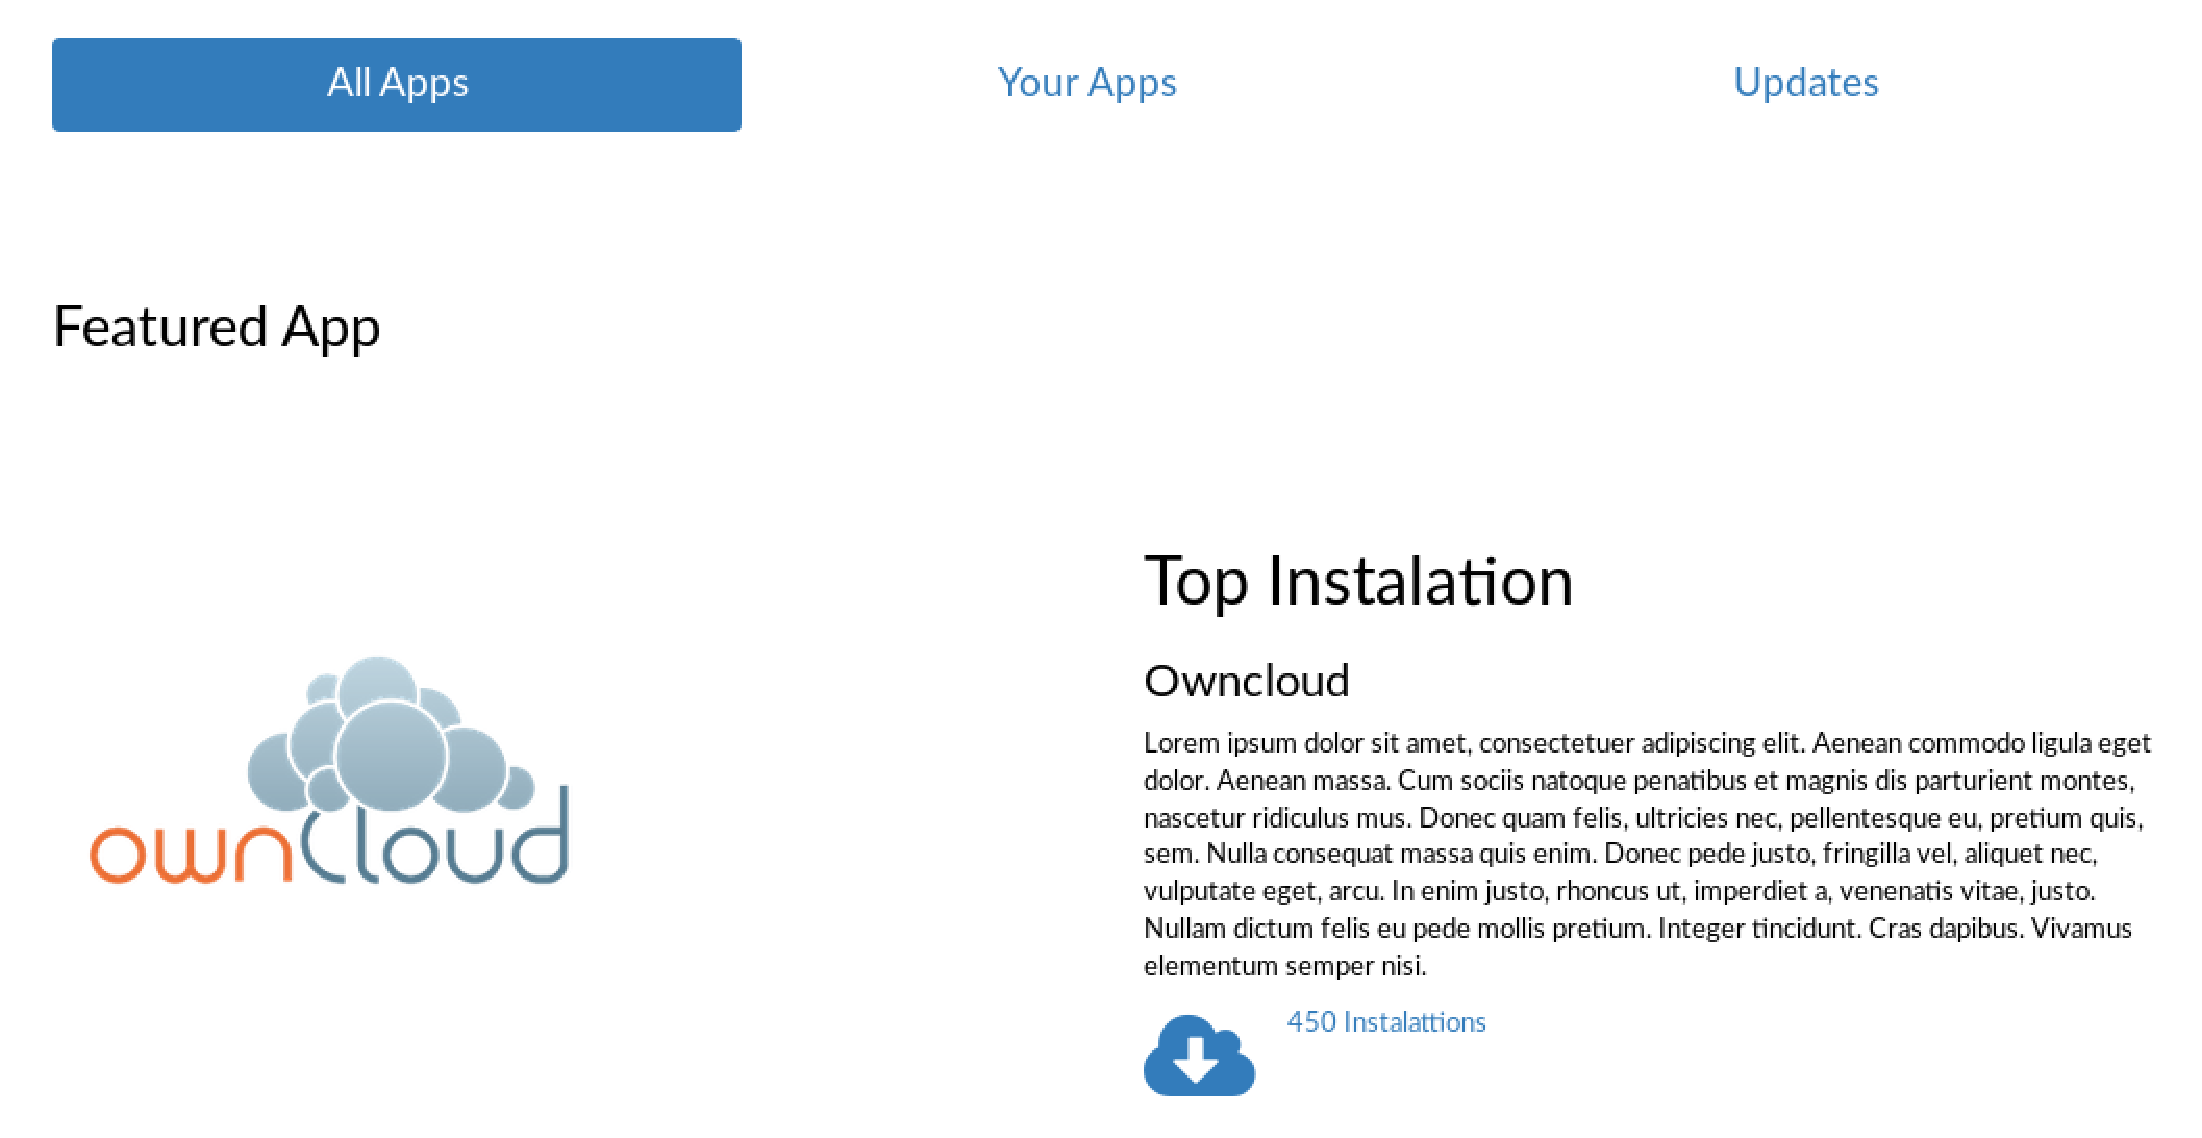
\includegraphics[width=0.8\textwidth]
      {figuras/shak1}
      \caption{Aplicação mais instalada pelo Shak}
  \label{fig:shakx1}
\end{figure}

\begin{figure}[H]
  \centering
  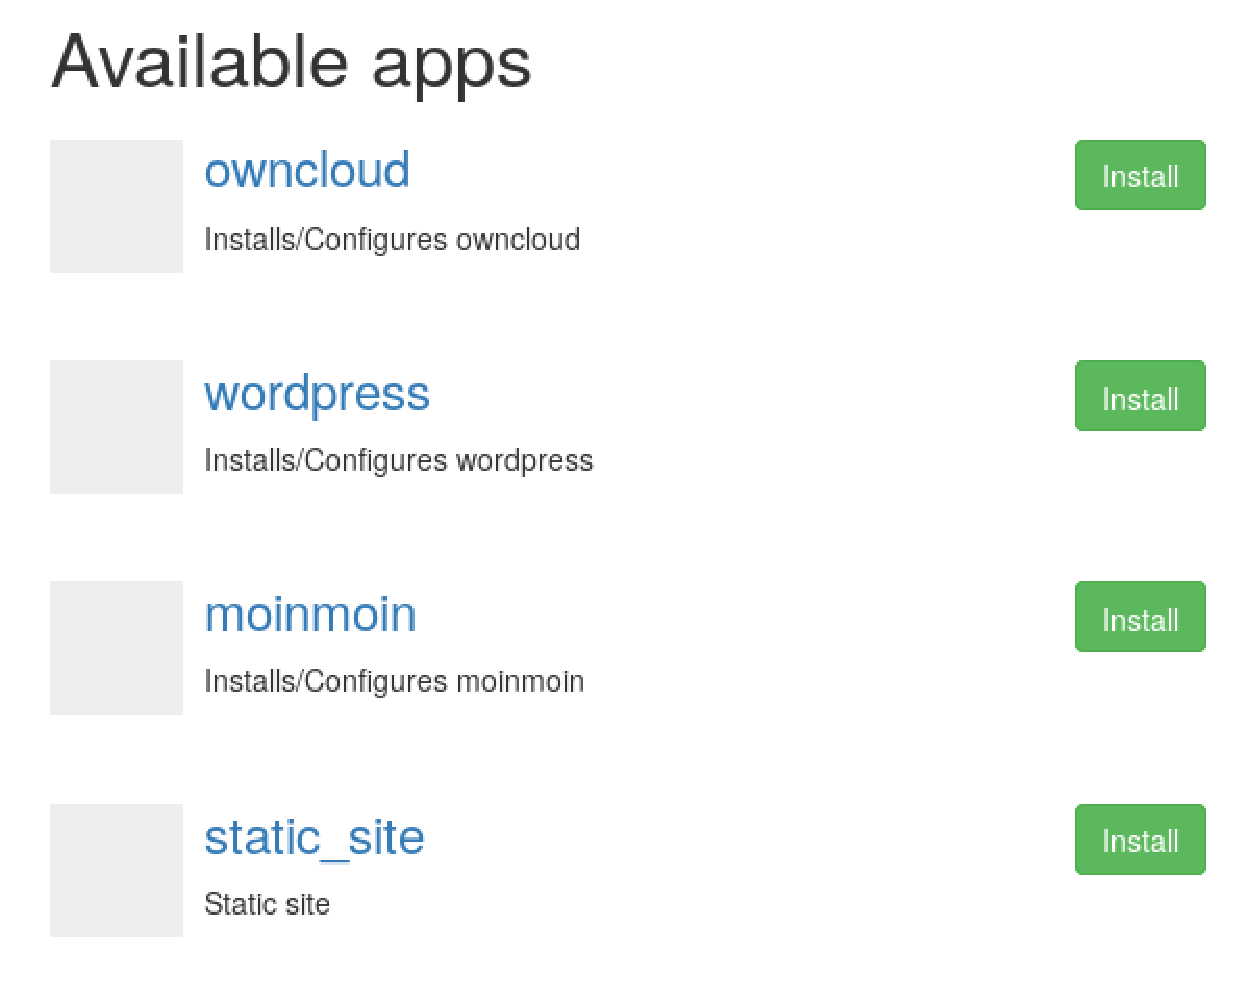
\includegraphics[width=0.6\textwidth]
      {figuras/shak1-2}
      \caption{aplicações disponíveis para instalação}
  \label{fig:shakx1.2}
\end{figure}

Ao selecionar uma aplicação para instalar, o usuário deverá informar as mesmas
informações que são necessárias na instalação via linha de comando. Na Figura \ref{fig:shakxx}
o usuário deve informar o endereço, o caminho da aplicação e confirmar.

\begin{figure}[h]
  \centering
  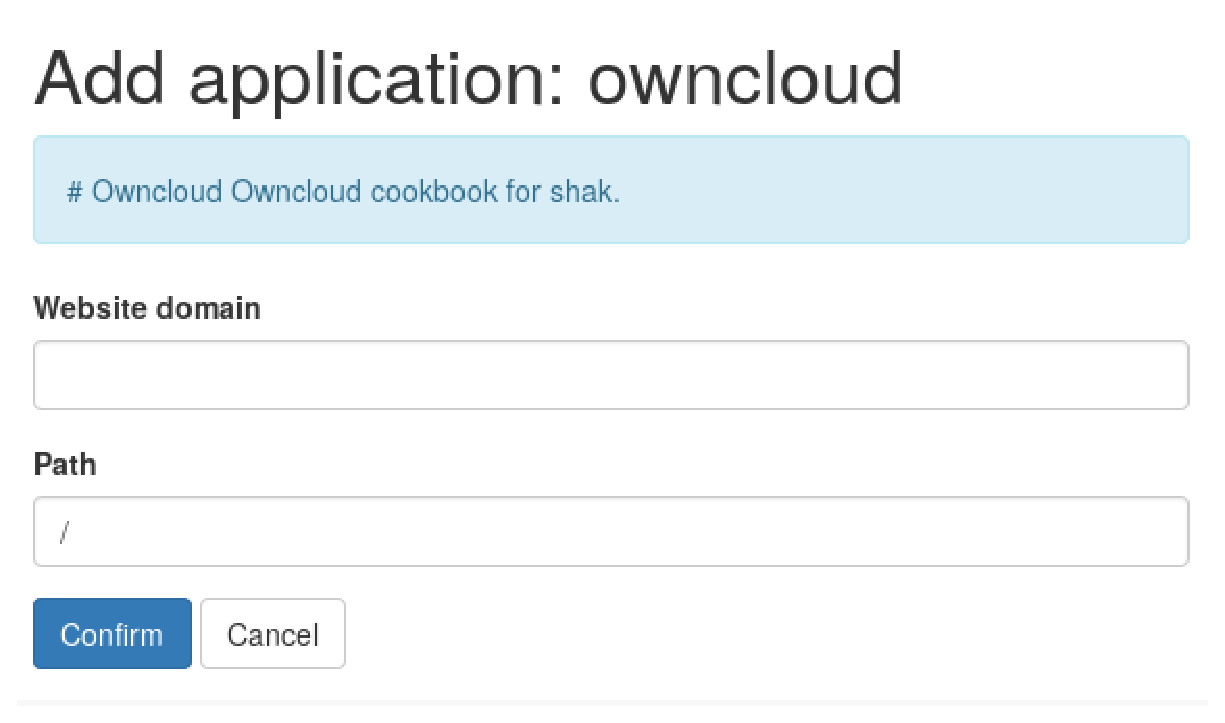
\includegraphics[width=0.6\textwidth]
      {figuras/shakx}
      \caption{Informações necessárias para implantar uma aplicação}
  \label{fig:shakxx}
\end{figure}

Na Figura \ref{fig:shakx2}, é onde o usuário pode ver suas aplicações instaladas e editar
suas informações.

\begin{figure}[H]
  \centering
  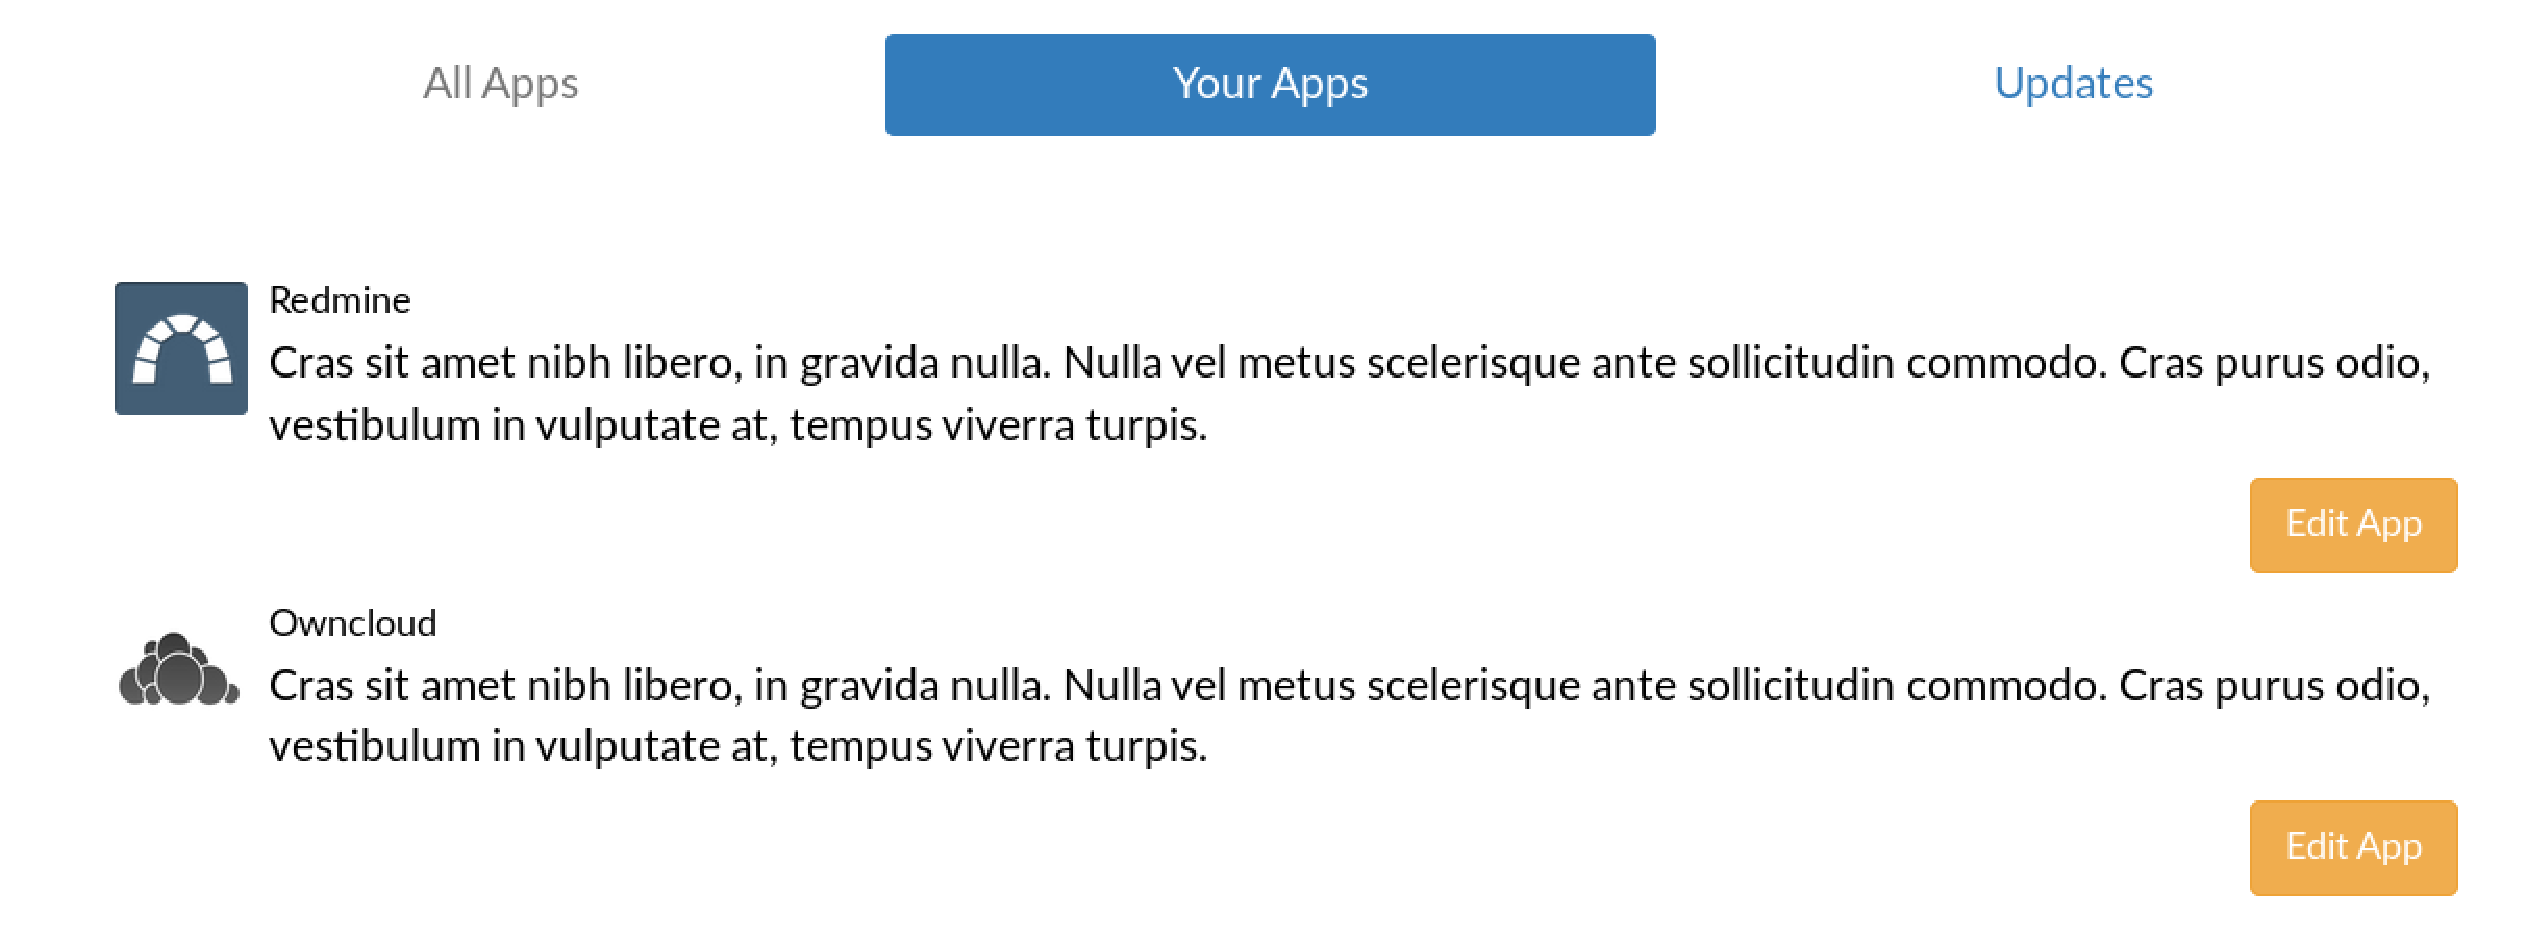
\includegraphics[width=0.8\textwidth]
      {figuras/shak2}
      \caption{Aplicações já instaladas pelo Shak}
    \label{fig:shakx2}
\end{figure}

Por fim, na Figura \ref{fig:shakx3}, é onde o usuário pode atualizar suas aplicações.

\begin{figure}[H]
  \centering
  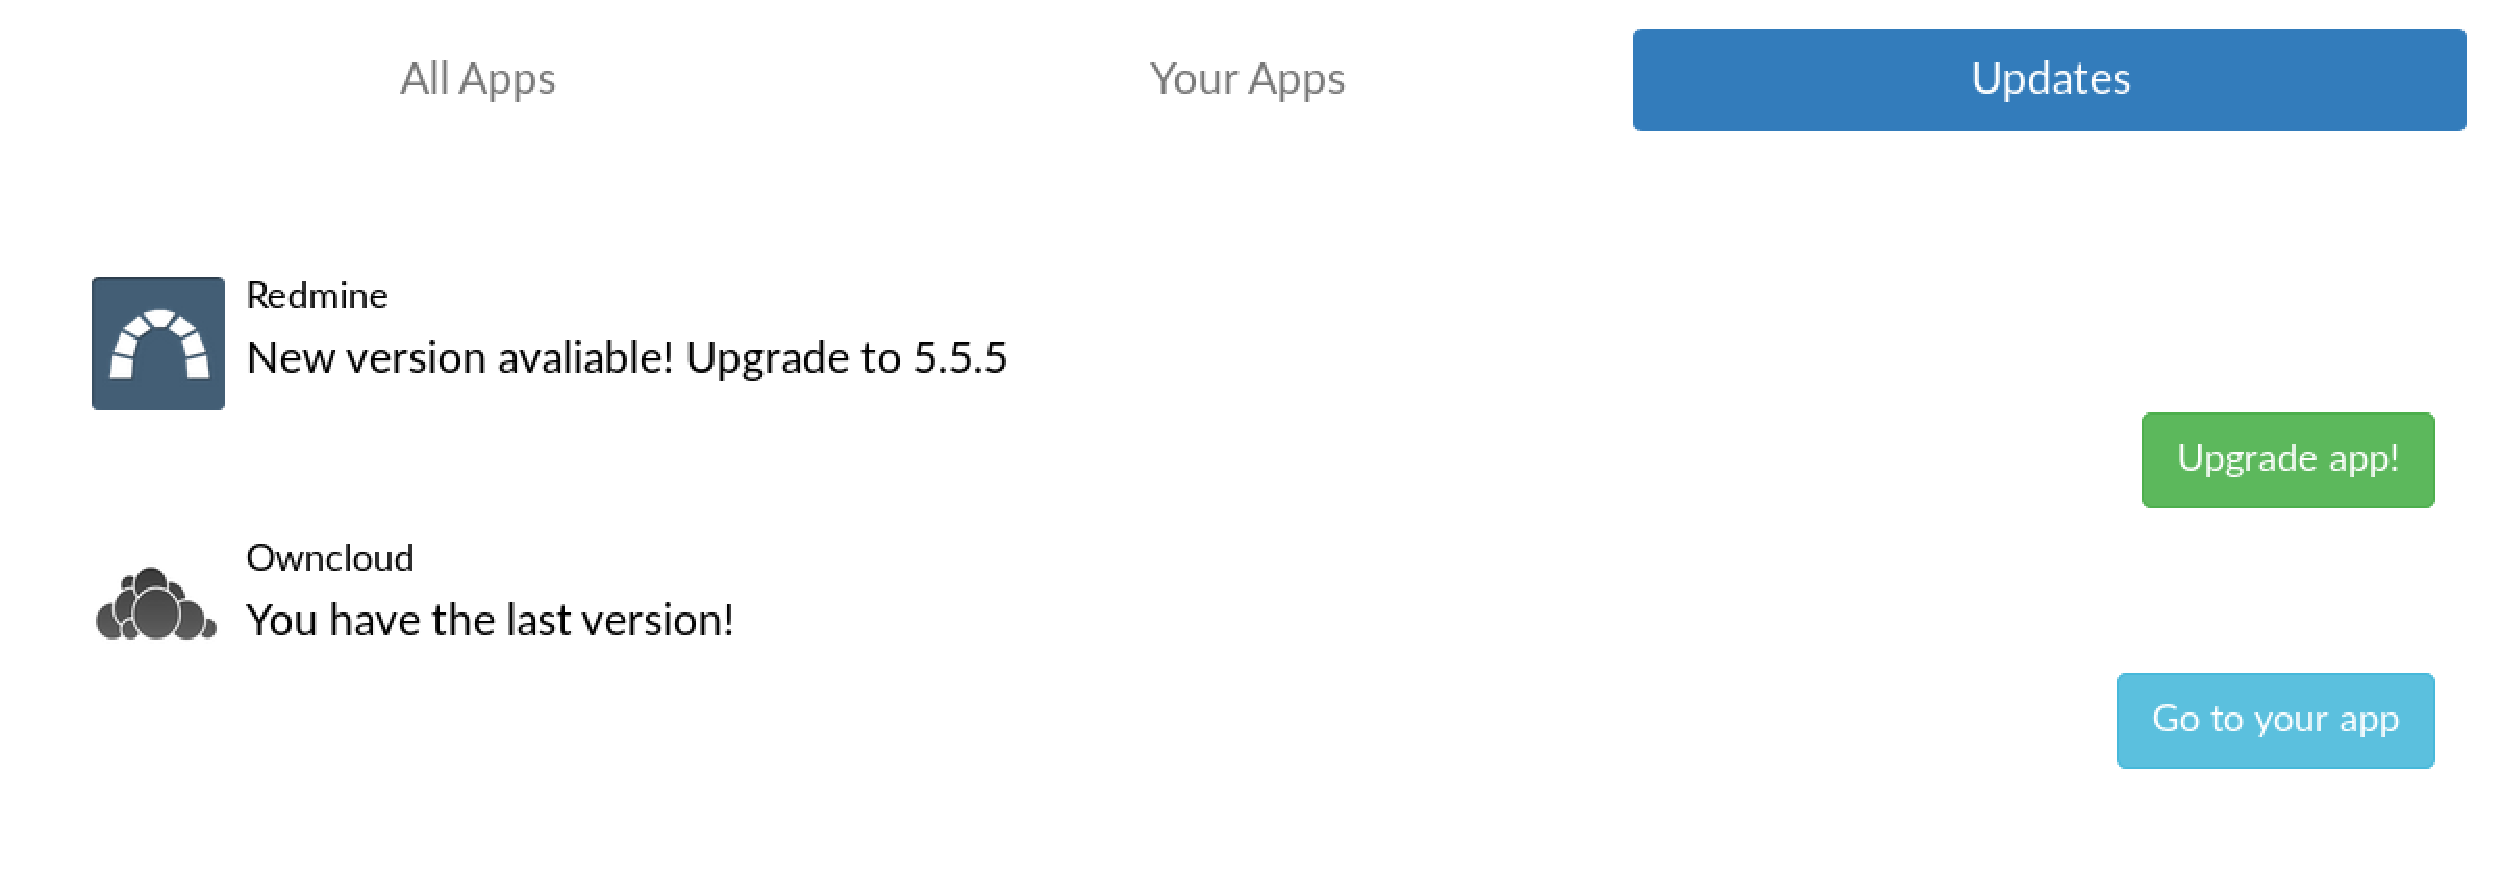
\includegraphics[width=0.8\textwidth]
      {figuras/shak3}
      \caption{Aplicações com atualizações disponíveis}
  \label{fig:shakx3}
\end{figure}

